%! Author = weiss
%! Date = 20.01.2025
\Author{\daAuthorThree}
    This chapter concentrates on exploring the Spring ecosystem and covers core components like Spring Framework, Spring Boot and Spring Data JPA. It highlights the advantages of this ecosystem in simplifying Java development and improving the efficiency.

    \subsection{Spring Boot}
    Spring Boot is a tool which makes developing web applications and microservices with the Java Spring Framework faster and easier. As powerful as the Spring Framework on its own is, it still requires much time and knowledge to configure, set-up and deploy Spring apps. Spring Boot tries to mitigate this effort with three features 

    \textbf{Autoconfigure:}
        \begin{itemize}
            \item Autoconfigure initializes Spring apps with a preset of dependencies so that the developer does not have to configure those manually. Spring Boot comes with this feature to automatically configure the Spring Framework and third-party packages based on the project requirements.
            \item Even though the developer can override the default configuration after the initialization, the initial setup makes the development process faster and more efficient.
            \item Meanwhile the autoconfiguration also reduces the possibility of many human errors which can occur during the configuration of an Java application.
        \end{itemize}
    \textbf{Opinionated Approach:}
        \begin{itemize}
            \item When adding and configuring startup dependencies, Spring Boot takes a subjective approach, customizing them to the requirements of the project. The right packages and default values are chosen automatically by Spring Boot, eliminating the need for human setup and decision-making for each configuration.

            \item During initialization, project requirements can be specified, allowing selection from a vast collection of starter dependencies, known as "Spring Starters," which cover most common use cases. For example, the "Spring Web" dependency simplifies the development of Spring-based web applications by including all necessary dependencies with minimal configuration. Likewise, "Spring Security" provides built-in authentication and access control features. 

            \item More than 50 official Spring Starters are offered by Spring Boot, and there are numerous other third-party starters accessible.


        \end{itemize}
    \textbf{Stand-Alone Application:}
        \begin{itemize}
            \item With the help of Spring Boot, applications can be developed that function without the need for an external web server. This is accomplished by immediately integrating a web server, such as Tomcat, with the application as it is initializing. As a result, the application can be launched with the appropriate command on any platform.
        \end{itemize}      
        \Autocite{Andi:SpringBoot1, Andi:SpringBoot2}          
    
    \textbf{Setting up a Spring Boot app:} \newline
    A Spring Boot project can be initialized quickly using the \textbf{Spring Initializr}. For a new Spring Boot-based project, the \textbf{Spring Initializr} can be opened, where the project details are filled in and a packaged project is downloaded as a.zip file. While initializing, a number of factors have to be chosen that determine the project structure, such as the programming language, the version of Spring Boot, and any other dependencies required to support development. \newline
    Depending on the IDE where the development is being performed, a Spring Boot project can be directly developed inside the IDE itself. Even this method supports the same amount of configuration to simplify the process of development. Not all IDEs are capable of creating a Spring Boot project out of the box, and sometimes a separate plugin needs to be installed.\Autocite{Andi:SpringInit}

    \begin{figure} [H]
        \centering
        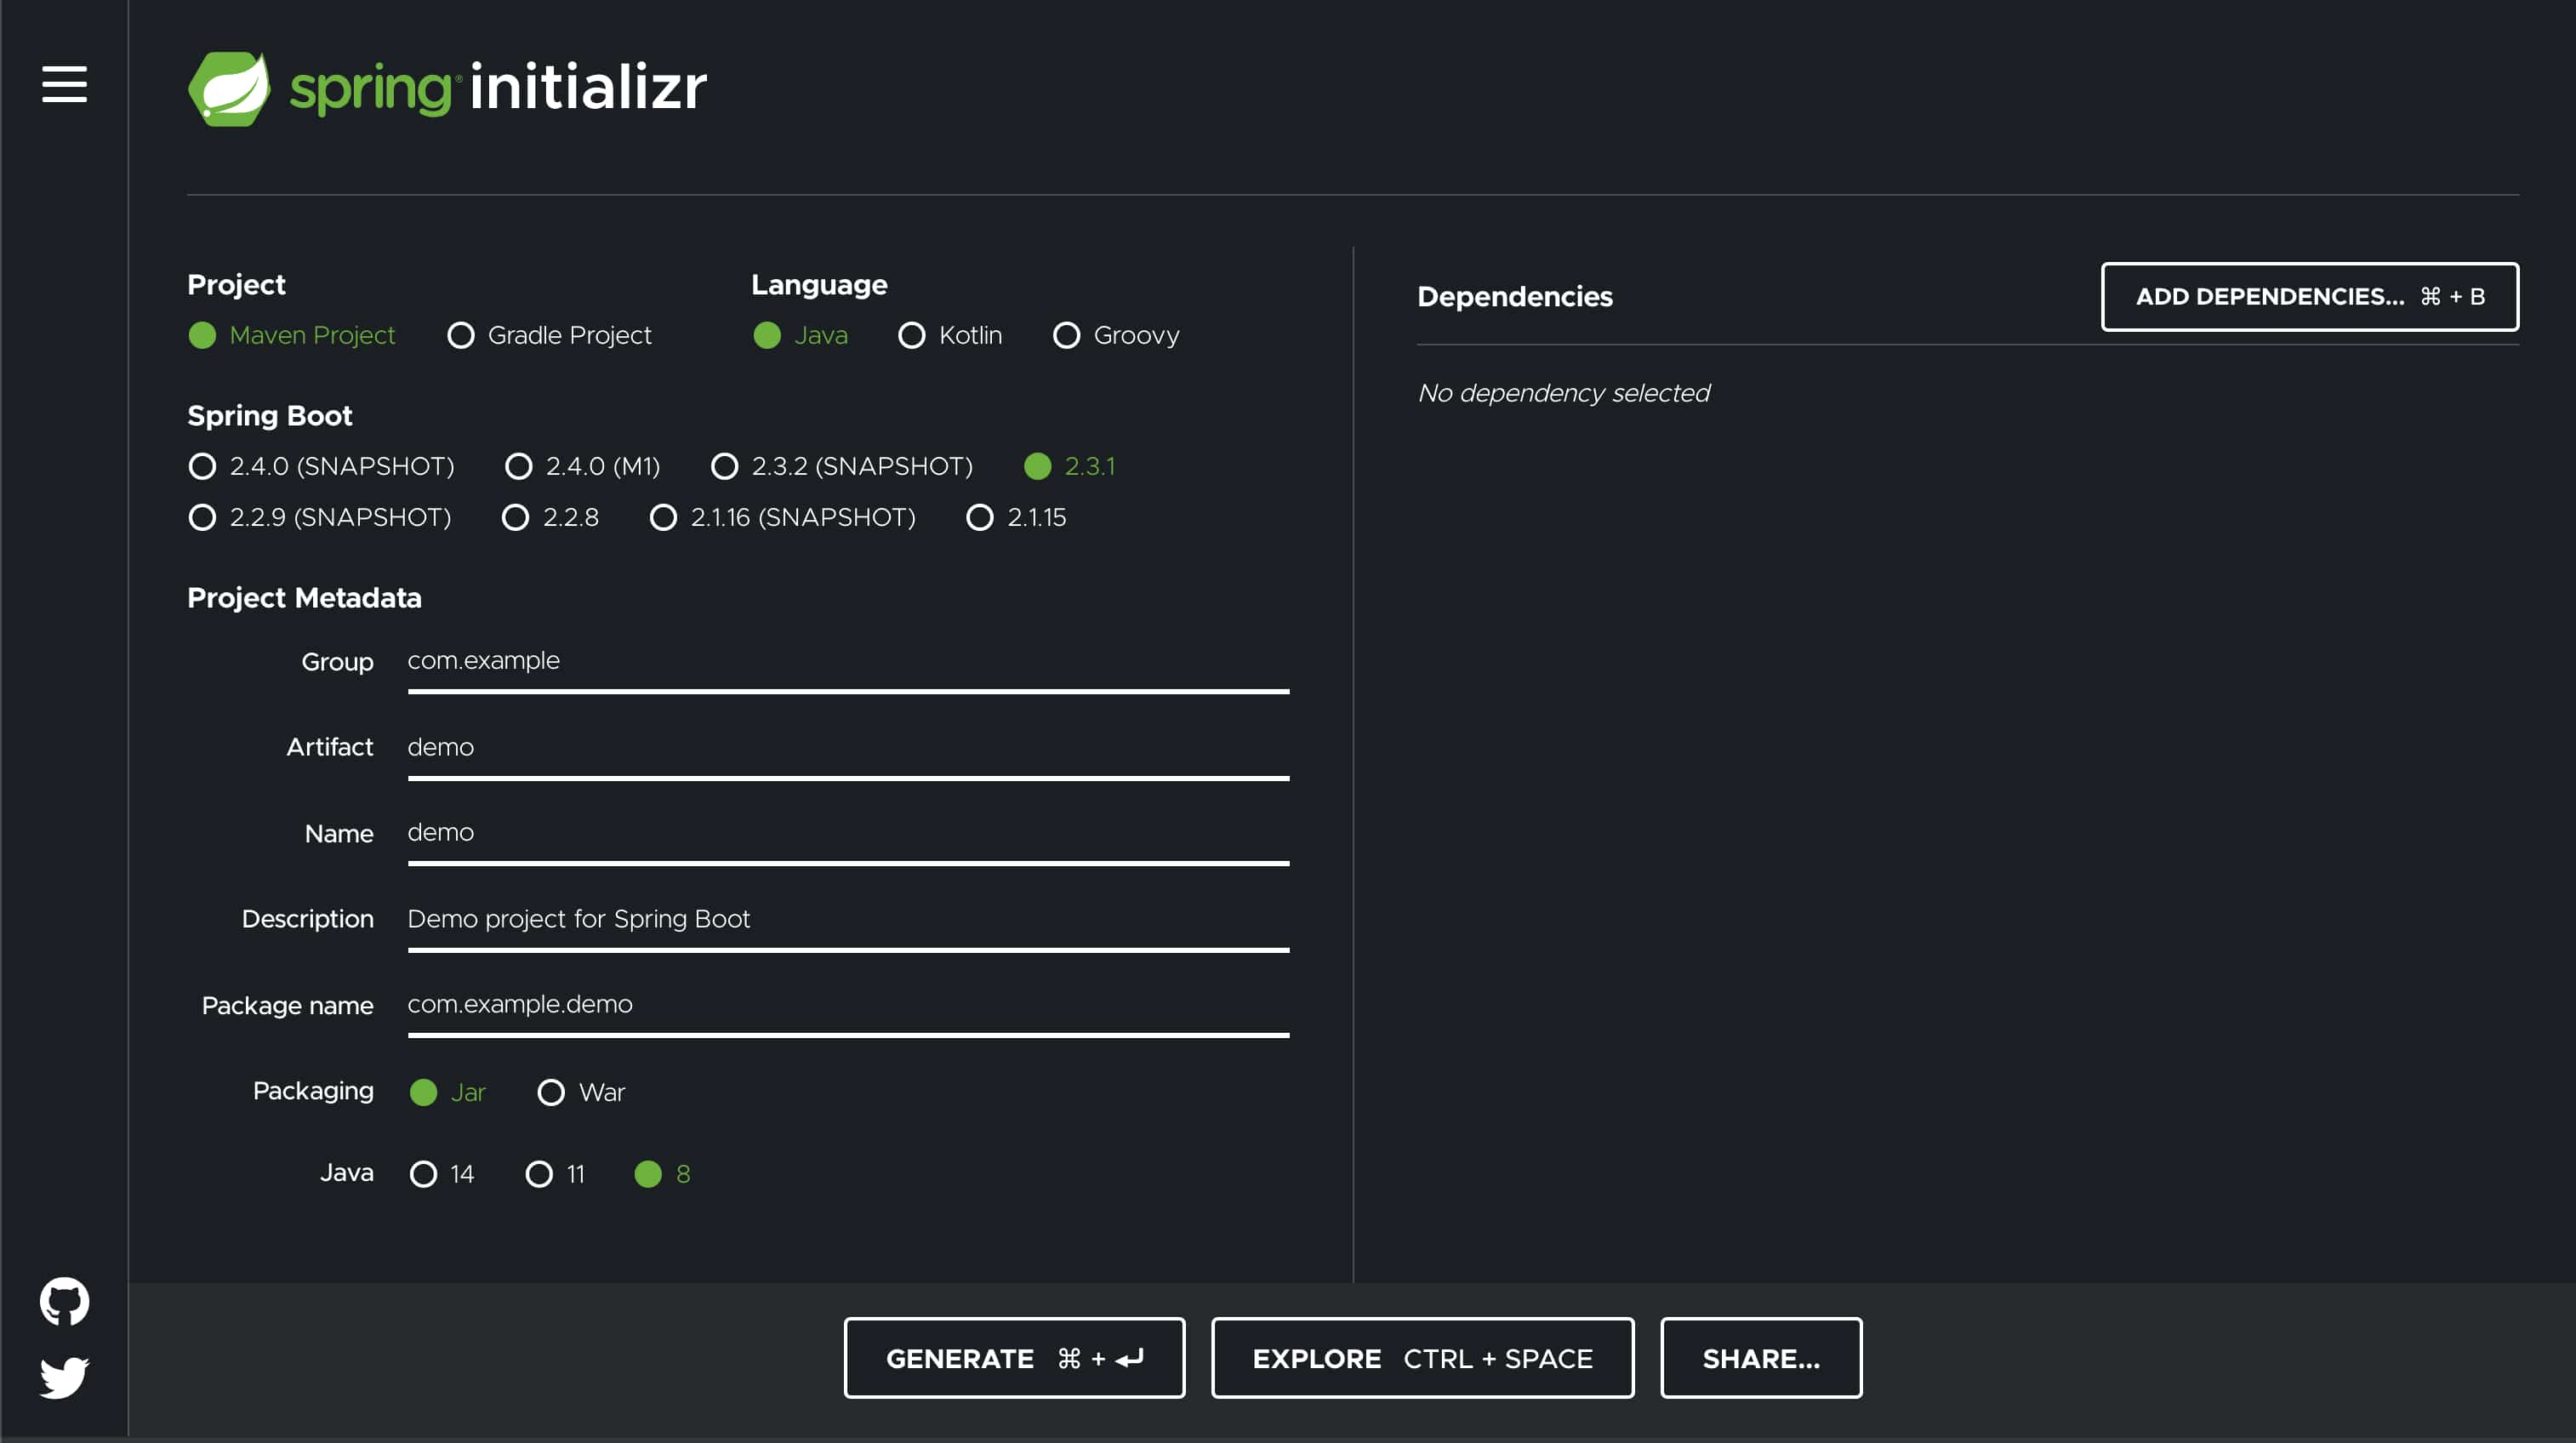
\includegraphics [width=1\textwidth] {images/andreas/springFramework/springInit.jpg}
        \caption{GUI of the Spring Initializr}
        \cite{Andi:SpringInit}
    \end{figure}
    
    \textbf{Difference between Spring Boot and Spring Framework:} \newline
    Spring Boot's greatest strengths over the standard Spring Framework are its simplicity and quicker development. Theoretically, this is at the expense of the higher degree of flexibility that direct Spring Framework usage would provide. Practically, the compromis is more than  worth it, as the Spring Framework's annotation system can still be utilized to inject other dependencies effectively. Besides, all Spring Framework functionalities like easy event handling and native security continue to be accessible. \Autocite{Andi:SpringBoot2}
    
    \subsection{Spring Data JPA}
    Spring Data JPA stands for Java Persistence API and provides a specification for persisting, reading and managing data from the object in the program, which are called entities, to project's tables in the database. JPA specifies a set of rules for developing interfaces that follow specific standards. As a result, JPA is just some guidelines to implement ORM.
    ORM is the process of persisting an object in java directly into a database table. \newline
    The goal of Spring Data JPA is to create classes called "Repositories" which significantly reduce the amount of unnecessary code to access and manipulate data from the database of a project. \newline 

    \textbf{Entities:} \newline
    As already mentioned, the object from which Spring Data JPA manages the data are called entities. Every table of a database is an entity with each attribute being a column in the respective table. The \texttt{@Entity} annotation can be used to define the entity, guaranteeing that the class is understood as a component of the database structure and handled appropriately. However, this annotation is not the only one which is supported by JPA. By using annotations such as \texttt{@Id} or \texttt{@GeneratedValue}, different custom features of the entity, and therefore the database table, can be defined. Those annotations are a way to make the development of the project much faster and even more efficient. \Autocite{Andi:Entity1, Andi:Entity2, Andi:Entity3} \newline

    \textbf{Data access object layer:} \newline
    Although there are many annotations that are usable for an entity, there is one annotation which is a core feature in JPA. The \texttt{@Repository} annotation is a marker for a class that fulfills the role of a repository which is also know as a Data Access Object. However, something else need to be done when using the \texttt{@Repository} annotation.
    When this annotation is used, the repository class must extend the \texttt{JpaRepository} class, which provides many built-in methods for managing, manipulating, sorting, and filtering data in the respective database table. If a required operation is not available by default, custom queries can also be defined within the repository class. \Autocite{Andi:Repo} \newline 

    \textbf{Service Layer:} \newline
    Classes that use the \texttt{@Service} annotation are used with classes that provide some data manipulation methods such as a repository-class. By implementing such a class, the project structure is better understandable and more clear to other developers which may work on this project later on. \Autocite{Andi:ServiceLayer1,Andi:ServiceLayer2}  \newline 

    \textbf{Controller Layer:} \newline
    This Layer provides the applications with the routes with which the data can get manipulated through a GUI. By using the \texttt{@RestController} annotation, an actual controller class can be defined. The controller uses the service classes from the service layer to get the data or manipulate it in any way. It also specifies the routes which the code can then
    access in any form of user interface so that the user can actually use or see the data.
    \Autocite{Andi:ControllerLayer} \newline

    \textbf{Mappings:} \newline
    There are numerous annotations that define routes along with all their features and how they can be accessed. The \texttt{@GetMapping} gives the user data in any form. This can be all the data from a table or a specific entry in a table based on any filter. The \texttt{@PostMapping} is used if a user would want to create a new entry in a specific table. \newline
    For example, in a company's management system, the \texttt{@PostMapping} annotation can be used to build a route for adding a new employee to the database. If the employee's address or surname were to change, the \texttt{@PutMapping} annotation would be used to update the stored data for that employee. On the other side, if the employee were to resign, the \texttt{@DeleteMapping} annotation would be used to enable the manager to remove the employee from the company's database. \newline
    These routes can then be accessed through a GUI, allowing the user to manage, update, or delete data as needed. \Autocite{Andi:JPA}
    
    \subsection{Lombok}
    In the modern days of Java development, one big challenge developers face is writing boilerplate code which are code segments that repeat itself over and over again and get used often in a project. This is especially the case in frameworks like Spring Boot where we use classes like the service layer that involve a significant amount of repetitive code.  \newline
    "Project Lombok" is a Java library that has the aim to reduce this boilerplate code by automatically generating the code for commonly used patterns. By integrating Lombok in your Spring Boot project, you can not only simplify your code but make it easier to read maintain and write. 
    Lombok works great with the whole Spring framework. If you would want to use a project with Spring Data JPA, you would not get that far without using any annotations provided by Project Lombok. To flag an entity class for Spring Data JPA, you need to use the \texttt{@Entity} annotation. This annotation comes from the Lombok library and adds a couple of 
    features to this class so that JPA recognizes it as an entity for the database. \newline
    Lombok injects the needed methods directly into the compiled class files when the program is getting build, which reduces the need to manually write common functions like constructors, getter and setters. When an annotation like \texttt{@Getter}, \texttt{@Setter}, \texttt{@AllArgsConstructor} is used, Lombok modifies the code before the compilation is done. This ensures that the generated methods are available at runtime while keeping the source code clean and minimal. \newline
    For example, using \texttt{@AllArgsConstructor} tells Lombok to generate a constructor with all the variables of a class. Another useful annotation is \texttt{@Data}, which combines many methods like the \texttt{@Getter} and \texttt{@Setter}. Using this annotation further reduces repetitive code. \newline
    Since Lombok creates these methods during the compilation process, developers can keep their code clean while still having fully functional classes. \Autocite{Andi:Lombok1, Andi:Lombok2, Andi:Lombok3}
    
    \subsection{Advantages}
    The Spring Framework has a range of advantages that make it a popular choice among developers. These benefits shorten the development process and help in designing scalable and maintainable apps. \newline \newline
    \textbf{Reduced Boilerplate Code:} \newline 
    A huge factor of the Spring framework is its abilty to reduce repetitive code segments. Mainly through the Lombok library, the Spring framework gives the developer many ways to exchange repetitive code with annotations. \newline  \newline
    \textbf{Enhanced Testability:} \newline
    With Spring's huge library of dependencies you can not only get dependencies which make the coding easier but the testing too. Some dependencies gave us mock data to test the backend endpoints easier.\newline \newline
    \textbf{Flexibility:} \newline
    The same thing that helped us testing, gave us and other projects the flexibility with which you can for example expand or change certain things in your project. This was extremely helpful for us because a certain requirement changed while we were developing the backend.\newline \newline
    \textbf{Consistency:} \newline
    Spring provides consistent programming and configurations models across many different types of applications. Whether you would want to develop a web application or a microservice, Spring offers a unified approach which improves developer productivity.\newline \newline
    \textbf{Improved Productivity:} \newline
    Tools like Spring Boot, which are part of the Spring ecosystem, significantly enhance developer productivity by providing better approaches to different problems and embedded servers. \Autocite{Andi:SpringBoot2} \newline 
    